\documentclass{scrartcl}

% neccesarry for style
\usepackage[english]{babel}
\usepackage[utf8]{inputenc}
\usepackage[T1]{fontenc}
\usepackage{lmodern}

% tools for text
\usepackage{csquotes}
\usepackage{url}
\usepackage{hyperref}

% graphics
\usepackage{graphicx}
\usepackage{xcolor}
\usepackage{tikz}

% maths
\usepackage{amsmath,amssymb,amstext,amsthm}

% programming
\usepackage{listings}

\usepackage{wasysym} %lightning

\input{required/settings.tex}
\input{required/commands.tex}

\renewcommand{\labelenumi}{\alph{enumi})}
\begin{document}
	\begin{center}
		\LARGE
		Information Integration -- Exercise 3 -- Gabriel Glaser
	\end{center}
	
	\section*{Task 1: Mediator-Wrapper Architecture}
	\begin{center}
		\hspace*{-0.3cm}
		\fbox{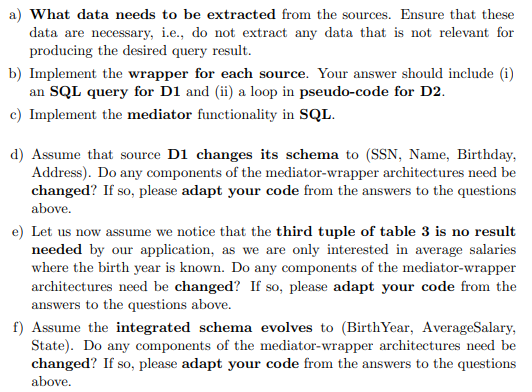
\includegraphics[width=1\textwidth]{figures/1_description.PNG}}
	\end{center}
	\begin{enumerate}
				\item\phantom{phantom}
		\begin{itemize}
			\item \textbf{D1}: Columns \textit{SSN} and \textit{Birthday}
			\item \textbf{D2}: Last two columns
		\end{itemize}
		
		\item\phantom{phantom}
		\begin{itemize}
			\item\textbf{Wrapper for D1}:
			\begin{center}
				\fbox{
					\begin{tabular}{l}
						\textbf{CREATE VIEW} WrapperTableD1 \textbf{AS}\\
						\hspace{0.5cm}\textbf{SELECT} SSN, Birthday \textbf{FROM} TableD1;\\
						\textbf{UPDATE} WrapperTableD1 \textbf{SET} Birthday = YEAR(Birthday);\\
						\textbf{ALTER} \textbf{TABLE} WrapperTableD1\\
						\hspace{0.5cm}\textbf{RENAME} \textbf{COLUMN} Birthday \textbf{TO} BirthYear;\\
					\end{tabular}
				}
			\end{center}
			\newpage
			\item\textbf{Wrapper for D2}:
			\begin{center}
				\fbox{
					\begin{tabular}{l}
						\textcolor{gray}{\# python-like script}\\
						run\_sql\_query(\\
						\hspace{0.5cm}\textbf{CREATE TABLE} WrapperTableD2 (\\
						\hspace{1cm}AverageSalary \textbf{INT}(255),\\
						\hspace{1cm}SSN \textbf{CHAR}(12)\\
						\hspace{0.5cm});\\
						)\\
						\textbf{for} row \textbf{in} \textit{csv\_rows}:\\
						\hspace{0.5cm}cells = row.split(",")\\
						\hspace{0.5cm}salary = \textbf{int}(remove\_last\_char(cells[4]))\\
						\hspace{0.5cm}ssn = cells[5]\\
						\hspace{0.5cm}run\_sql\_query(\\
						\hspace{1cm}\textbf{INSERT INTO} WrapperTableD2\\
						\hspace{1.5cm}\textbf{VALUES}(salary, ssn)\\
						\hspace{1cm});\\
						\hspace{0.5cm})
					\end{tabular}
				}
			\end{center}
		\end{itemize}
		
		\item \textbf{Mediator}:
		\begin{center}
			\fbox{
				\begin{tabular}{l}
					\textbf{CREATE} \textbf{VIEW} tmp \textbf{AS}\\
					\hspace{0.5cm}\textbf{SELECT} * \textbf{FROM} WrapperTableD1, WrapperTableD2\\
					\hspace{0.5cm}\textbf{WHERE} WrapperTableD1.SSN = WrapperTableD2.SSN;\\
					\textbf{CREATE} \textbf{VIEW} IntegratedTable \textbf{AS}\\
					\hspace{0.5cm}\textbf{SELECT} BirthYear, AverageSalary \textbf{FROM} tmp;
				\end{tabular}
			}
		\end{center}
		
		\item Nothing has to be changed, because the label of all relevant attributes didn't change.
		Therefore, the Wrapper for \textit{D1} remains to correctly return a table with birthyears and ssns.
		
		\item This requires a change which, for instance, can be implemented in the mediator by adding another condition to the join of both wrapper tables.
		The change has the semantic that requires the birthyear being non null, i.e.,
		\begin{center}
			\textbf{AND} WrapperTableD1.BirthYear \textbf{IS} \textbf{NOT} \textbf{NULL}.
		\end{center}
		
		\item So far, the integrated table doesn't contain the column \textit{State}, thus it has to be added (in the mediator):
		\begin{center}
			\textbf{ALTER} \textbf{TABLE} IntegratedTable \textbf{ADD} State \textbf{INT}(255);.
		\end{center}
	\end{enumerate}
	
	\section*{Task 2: Stable Marriage Algorithm}
	\begin{center}
		\hspace*{-0.3cm}
		\fbox{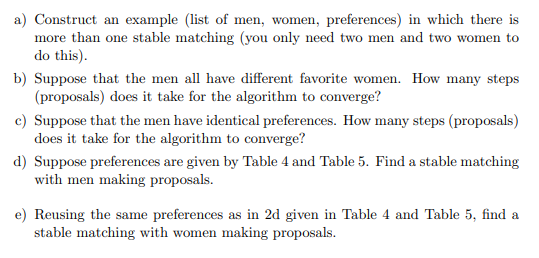
\includegraphics[width=1\textwidth]{figures/2_description.PNG}}
	\end{center}
	\begin{enumerate}
		\item\phantom{phantom}
		\begin{center}
			\begin{tabular}{c|c}
				Men & Women\\
				\hline
				A: 1, 2 & 1: A, B\\
				B: 1, 2 & 2: A. B
			\end{tabular}
		\end{center}
		\begin{itemize}
			\item (A,1) \& (B,2) is stable, because A doesn't prefer 2 and 1 doesn't prefer B.
			\item Similarly (B,1) \& (A,2) is stable, because B doesn't prefer 2 and 2 doesn't prefer B.
		\end{itemize}
		
		\item The algorithm needs exactly as many steps as men are there.
		This is because, during the algorithm each man will propose to a woman who didn't have an offer before.
		Thus, she accepts and also, won't get further proposals which may could lead to a change (break up and new search for the man who lost the woman who he initially proposed to).
		
		\item Let's assume each man $m_i$ has the priority list $(w_1, w_2, ..., w_n)$.
		It is the case that each man $m_i$ performs at least 1, but at most $n$ proposals.
		Also, it is not possible that any two men $m_i, m_j, i\neq j$ have the same amount of proposals, because then both of their last proposal would address the same woman (which is not allowed).
		The only way of distributing the (pair-wise different) number of proposals of $n$ men would be that
		\begin{itemize}
			\item one man has 1 proposal
			\item one man has 2 proposals
			\item one man has 3 proposals
			\item ...
			\item one man has $n$ proposals
		\end{itemize}
		Therefore, there are
		\[\sum_{i=1}^ni=\frac{n(n+1)}{2}\]
		proposals.
		
		\item\phantom{phantom}
		\begin{center}
			\begin{tabular}{|l|}
				\hline
				Adam $\to$ Beth $\surd$\\\hline
				Bill $\to$ Diane $\surd$\\\hline
				Carl $\to$ Beth $\surd$ $\quad$ Adam loses partner\\\hline
				Adam $\to$ Amy $\surd$\\\hline
				Dan $\to$ Amy \lightning\\\hline
				Dan $\to$ Diane $\surd$ $\quad$ Bill loses partner\\\hline
				Bill $\to$ Beth \lightning\\\hline
				Bill $\to$ Amy \lightning\\\hline
				Bill $\to$ Cara $\surd$\\\hline
				Eric $\to$ Beth \lightning\\\hline
				Eric $\to$ Diane $\surd$ $\quad$ Dan loses partner\\\hline
				Dan $\to$ Cara \lightning\\\hline
				Dan $\to$ Beth \lightning\\\hline
				Dan $\to$ Ellen $\surd$\\
				\hline
			\end{tabular}
		\end{center}
		(Each arrow represents a proposal which may be accepted $\surd$ or rejected \lightning)\\
		\textit{Result}: (Adam, Amy), (Bill, Cara), (Carl, Beth), (Dan, Ellen), (Eric, Diane).
		
		\item\phantom{phantom}
		\begin{center}
			\begin{tabular}{|l|}
				\hline
				Amy $\to$ Eric $\surd$\\\hline
				Beth $\to$ Carl $\surd$\\\hline
				Cara $\to$ Bill $\surd$\\\hline
				Diane $\to$ Adam $\surd$\\\hline
				Ellen $\to$ Dan $\surd$\\
				\hline
			\end{tabular}
		\end{center}
	Result: (Amy, Eric), (Beth, Carl), (Cara, Bill), (Diane, Adam), (Ellen, Dan).
		
	\end{enumerate}
	\newpage
	\section*{Task 3: Schema Matching}
	\begin{center}
		\hspace*{-0.3cm}
		\fbox{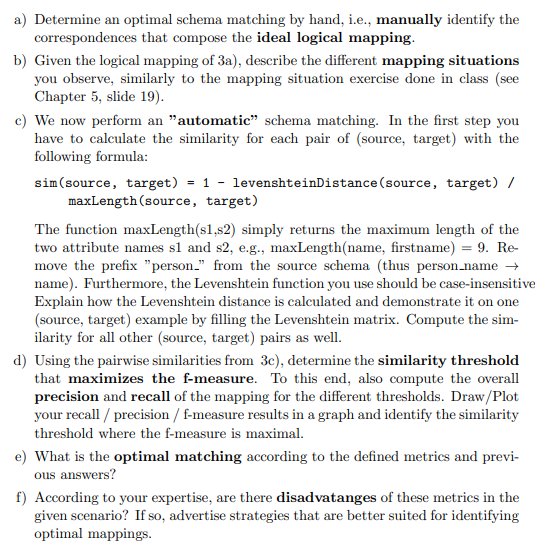
\includegraphics[width=0.9\textwidth]{figures/3_description.PNG}}
	\end{center}
	\begin{enumerate}
		\item Optimal Schema:
		\begin{center}
			\fbox{
				\begin{tabular}{l}
					<element name="person">\\
					\hspace{0.5cm}<element name="name" type="xsd:string"/>\\
					\hspace{0.5cm}<element name="birthDate" type="xsd:date"/>\\
					\hspace{0.5cm}<element name="birthPlace" type="xsd:string"/>\\
					\hspace{0.5cm}<element name="address" type="xsd:string"/>\\
					\hspace{0.5cm}<element name="phoneNumber" type="xsd:string"/>\\
					\hspace{0.5cm}<element name="emailAddress" type="xsd:string"/>\\
					</element>
				\end{tabular}
			}
		\end{center}
		Preserves all information from both schemas while keeping the effort for data fusion low.
		For instance, \textit{name} from schema 1 can be directly written to an instance of the global schema and \textit{firstName}, \textit{lastName} can be easily transformed accordingly. Similarly, \textit{address} of schema 2 can be directly written and the distinguished address components in schema 1 can be easily transformed accordingly.
		
		\item\phantom{phantom}
		\begin{center}
			\hspace*{-4cm}
			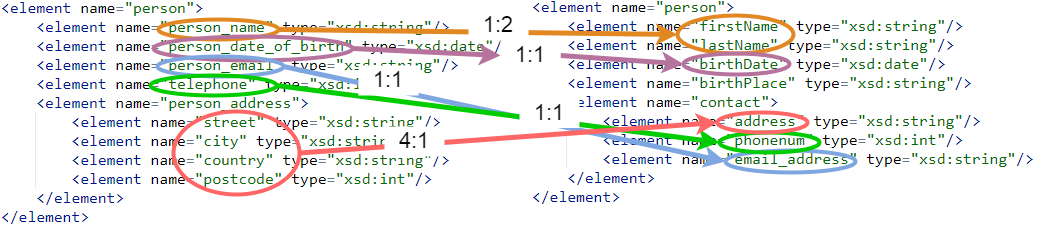
\includegraphics[width=1.5\textwidth]{figures/3b.png}
		\end{center}
		
		\item Illustration of Levenshtein(\textit{phonenum}, \textit{telephone}):
			\begin{center}
				\large
				\begin{tabular}{|c|c|c|c|c|c|c|c|c|c|c|}
					\hline
					  &   & t & e & l & e & p & h & o & n & e\\\hline
					  & 0 & 1 & 2 & 3 & 4 & 5 & 6 & 7 & 8 & 9\\\hline
					p & 1 & 1 & 2 & 3 & 4 & 4 & 5 & 6 & 7 & 8\\\hline
					h & 2 & 2 & 2 & 3 & 4 & 5 & 4 & 5 & 6 & 7\\\hline
					o & 3 & 3 & 3 & 3 & 4 & 5 & 5 & 4 & 5 & 6\\\hline
					n & 4 & 4 & 4 & 4 & 4 & 5 & 6 & 5 & 4 & 5\\\hline
					e & 5 & 5 & 4 & 5 & 4 & 5 & 6 & 6 & 5 & 4\\\hline
					n & 6 & 6 & 5 & 5 & 5 & 5 & 6 & 6 & 6 & 5\\\hline
					u & 7 & 7 & 6 & 6 & 6 & 6 & 6 & 7 & 7 & 6\\\hline
					m & 8 & 8 & 7 & 7 & 7 & 7 & 7 & 7 & 8 & 7\\\hline
				\end{tabular}
			\end{center}
		\begin{itemize}
			\item Each entry of the matrix above represents the number of character-operations (insert, replace, remove) needed to transform the top prefix to the left prefix.
			
			\item Therefore, the first row/column can be initialized with 0, 1, 2 etc., because they represent the number of operations to transform the empty string to the respective prefix.
			
			\item Furthermore, to transform the prefixes of cell $(i,j)$ into each other, either
			\begin{itemize}
				\item Take previous shorter prefix (cell above) plus an insert operation.
				\item Take longer prefix (cell left) plus a remove operation.
				\item Take prefix of same length (cell diagonal top-left) plus a replace operation. The plus one is not necessary, if the characters the the cell already are equal.
			\end{itemize}
			
			\item Applying this yields a table like above while the bottom-right value represents the final distance measure.
		\end{itemize}
		Therefore, the Levenshtein distance in example is 7.\\
		Thus, sim(\textit{phonenum}, \textit{telephone}) = $1-\frac{7}{\max\{|\textit{phonenum}|, |\textit{telephone}|\}}=1-\frac{7}{9}=\frac{2}{9}$
		
		Remaining similarities:
		\begin{center}
			\begin{tabular}{|c|c|c|}
				\hline
				source & target & sim\\
				\hline
				name & firstName & 0.444\\
				name & lastName & 0.5\\
				name & birthDate & 0.222\\
				name & birthPlace & 0.199\\
				name & address & 0.142\\
				name & phonenum & 0.125\\
				name & email\_address & 0.153\\
				date\_of\_birth & firstName & 0.0\\
				date\_of\_birth & lastName & 0.076\\
				date\_of\_birth & birthDate & 0.076\\
				date\_of\_birth & birthPlace & 0.0\\
				date\_of\_birth & address & 0.076\\
				date\_of\_birth & phonenum & 0.076\\
				date\_of\_birth & email\_address & 0.076\\
				email & firstName & 0.111\\
				email & lastName & 0.125\\
				email & birthDate & 0.111\\
				email & birthPlace & 0.099\\
				email & address & 0.0\\
				email & phonenum & 0.0\\
				email & email\_address & 0.384\\
				\hline
			\end{tabular}
			\hfill
			\begin{tabular}{|c|c|c|}
				\hline
				source & target & sim\\
				\hline
				telephone & firstName & 0.111\\
				telephone & lastName & 0.111\\
				telephone & birthDate & 0.111\\
				telephone & birthPlace & 0.199\\
				telephone & address & 0.0\\
				telephone & phonenum & 0.222\\
				telephone & email\_address & 0.153\\
				street & firstName & 0.222\\
				street & lastName & 0.25\\
				street & birthDate & 0.222\\
				street & birthPlace & 0.099\\
				street & address & 0.285\\
				street & phonenum & 0.125\\
				street & email\_address & 0.153\\
				city & firstName & 0.222\\
				city & lastName & 0.125\\
				city & birthDate & 0.222\\
				city & birthPlace & 0.199\\
				city & address & 0.0\\
				city & phonenum & 0.0\\
				city & email\_address & 0.076\\
				\hline
			\end{tabular}
			\\
			\vspace{0.3cm}
			\begin{tabular}{|c|c|c|}
				\hline
				source & target & sim\\
				\hline
				country & firstName & 0.111\\
				country & lastName & 0.125\\
				country & birthDate & 0.0\\
				country & birthPlace & 0.0\\
				country & address & 0.0\\
				country & phonenum & 0.125\\
				country & email\_address & 0.076\\
				postcode & firstName & 0.333\\
				postcode & lastName & 0.375\\
				postcode & birthDate & 0.222\\
				postcode & birthPlace & 0.199\\
				postcode & address & 0.0\\
				postcode & phonenum & 0.125\\
				postcode & email\_address & 0.153\\
				\hline
			\end{tabular}
		\end{center}
		
		\item Assume ground truth:
		\begin{itemize}
			\item date\_of\_birth = birthDate
			\item email = email\_address
			\item telephone = phonenum
		\end{itemize}
		Other mappings are considered wrong, because either the mapping is not 1:1 or they have different semantics.
		Furthermore, all possible thresholds for all similarity values which need to be tested are all different ones retrieved in the task before (which are 16 similarities).
		\begin{center}
			\hspace*{-2.5cm}
			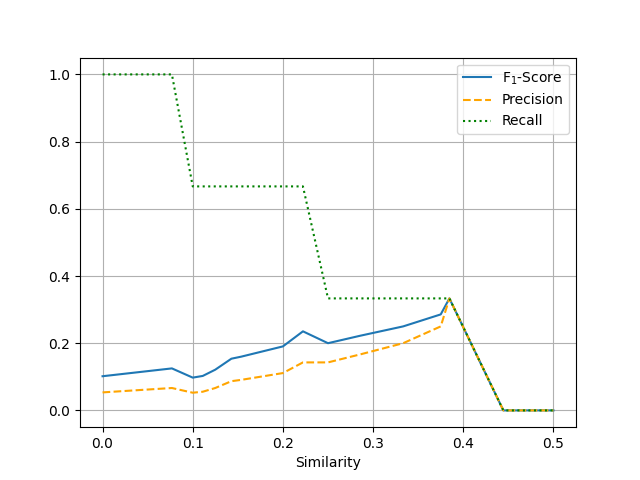
\includegraphics[width=1.25\textwidth]{figures/3d_x.png}
		\end{center}
		$\Rightarrow$ Best similarity threshold is $\approx0.39$.
		\begin{center}
			\begin{tabular}{c|c|c}
				& should be mapped & shouldn't be mapped\\\hline
				were mapped & TP & FP\\\hline
				weren't mapped & FN & TN\\
			\end{tabular}
		\end{center}
		\begin{itemize}
			\item\textit{Precision}: $\frac{TP}{TP + FP}$, i.e., proportion of how many mappings were correct.
			\item\textit{Recall}: $\frac{TP}{TP + FN}$, i.e., proportion of how many mappings were found, in comparison to the number of possible correct mappings.
			\item \textit{F$_1$} = $\frac{2PR}{P+R}$
		\end{itemize}
	
		\item name = lastName\\
		email = email\_address\\
		postcode = firstName (actually, lastName had a higher similarity, but not available for mapping)
		
		\item Using Levenshtein can be bad when equivalent attributes contain substrings at different word position, e.g., \enquote{telephone} and \enquote{phonenum}.
		An improved strategy could be to check whether one attribute label has a substring longer than, e.g., half or $\frac{1}{3}$ of the word and is part of the other attribute label string.
	\end{enumerate}
\end{document}
